\documentclass{article}
\usepackage{graphicx,lscape,enumitem,fullpage,wasysym,amsmath}
\usepackage[comma]{natbib}
\setcitestyle{aysep={}}
\title{Statistics for fission track thermochronology}

\author{Pieter Vermeesch\\London Geochronology Centre\\University
  College London}

\renewcommand{\thesection}{6.\arabic{section}}
\renewcommand{\thesubsection}{6.\arabic{section}.\arabic{subsection}}
\renewcommand{\theequation}{6.\arabic{equation}}
\renewcommand\thefigure{6.\arabic{figure}}
\renewcommand\thetable{6.\arabic{table}}
\renewcommand{\figurename}{Fig.}

\begin{document}

\maketitle

\begin{abstract}
This Chapter introduces statistical tools to extract geologically
meaningful information from fission-track (FT) data using both the
external detector and LA-ICP-MS methods. The spontaneous fission of
$^{238}$U is a Poisson process resulting in large single grain age
uncertainties. To overcome this imprecision, it is nearly always
necessary to analyse multiple grains from a single sample. The degree
to which the analytical uncertainties can explain the observed scatter
of the single grain data can be visually assessed on a radial plot,
and objectively quantified by a Chi-square test. For sufficiently low
values of the Chi-square statistic (or sufficiently high p-values),
the pooled age of all the grains gives a suitable description of the
underlying `true' age population. Samples may fail the Chi-square test
for several reasons. A first possibility is that the true age
population does not consist of a single discrete age component, but is
characterised by a continuous range of ages. In this case, a `random
effects' model can constrain the true age distribution using two
parameters: the `central age' and the `(over)dispersion'. A second
reason why FT datasets might fail the Chi-square test is if they are
underlain by multimodal age distributions. Such distributions may
consist of discrete age components, continuous age distributions, or a
combination of the two. Formalised statistical tests such as
Chi-square can be useful in preventing overfitting of relatively small
datasets. However, they should be used with caution when applied to
large datasets (including length measurements) which generate
sufficient statistical `power' to reject any simple yet geologically
plausible hypothesis.
\end{abstract}

\section{Introduction}

$^{238}$U is the heaviest naturally occurring nuclide in the Solar
System. Like all nuclides heavier than $^{208}$Pb, it is physically
unstable and undergoes radioactive decay to smaller, more stable
nuclides. 99.9998\% of the $^{238}$U nuclei shed weight by
disintegrating into eight He-nuclei ($\alpha$-particles) and a
$^{206}$Pb atom, forming the basis of the U-Pb and U-Th-He clocks. The
remaining 0.0002\% of the $^{238}$U undergoes spontaneous fission,
forming the basis of FT geochronology \citep{price1963,
  fleischer1965}. Because spontaneous fission of $^{238}$U is such a
rare event, the surface density of fission tracks (in counts per unit
area) is 10-11 orders of magnitude lower than the molar abundances of
$^{238}$U and $^4$He, respectively.  So whereas the U-Pb and (U-Th)/He
methods are based on mass spectrometric analyses of billions of Pb and
He atoms, FT ages are commonly based on manual counts of at most a few
dozen features. Due to these low numbers, the FT method is a low
precision technique. Whereas the analytical uncertainty of U-Pb and
(U-Th)/He ages is expressed in \% or \permil-units, it is not uncommon
for single-grain FT age uncertainties to exceed 10\% or even 100\%
(Sect.~\ref{sec:EDM}). Early attempts to quantify these uncertainties
\citep{mcgee1979,johnson1979} were criticised by
\citet{green1981a,green1981b}, who subsequently engaged in a fruitful
collaboration with two statisticians --Geoff Laslett and Rex
Galbraith-- to eventually solve the problem. Thanks to the combined
efforts of the latter two people, it is fair to say that the
statistics of the FT method are better developed than those of any
other geochronological technique. Several statistical tools that were
originally developed for the FT method have subsequently found
applications in other dating methods. Examples of this are the radial
plot (Sect.~\ref{sec:visualisation}), which is routinely used in
luminescence dating \citep{galbraith2010}, random effects models
(Sect.~\ref{sec:randomeffects}), which have been generalised to
(U-Th)/He \citep{vermeesch2010a} and U-Pb dating \citep{rioux2012},
and finite mixture models (Sect. \ref{sec:mixtures}), which were
adapted for detrital U-Pb geochronology \citep{sambridge1994}.\\

The statistical analysis of fission tracks is a rich and diverse
field, and this short Chapter cannot possibly cover all its
intricacies. Numerate readers are referred to the book by
\citet{galbraith2005}, which provides a comprehensive, detailed, and
self-contained review of the subject, from which the present Chapter
heavily borrows.  The Chapter comprises five Sections, which address
statistical issues of progressively higher order. Sect.~\ref{sec:EDM}
introduces the FT age equation using the External Detector Method
(EDM), which offers the most straightforward and elegant way to
estimate single-grain age uncertainties, even in grains without
spontaneous fission tracks.  Section \ref{sec:visualisation} compares
and contrasts different ways to visually represent multi-grain
assemblages of FT data, including kernel density estimates, cumulative
age distributions, and radial plots.  Sect.~\ref{sec:summarystats}
reviews the various ways to estimate the `average' age of such
multi-grain assemblages, including the arithmetic mean age, the pooled
age, and the central age. This Section will also introduce a
Chi-square test for age homogeneity, which is used to assess the
extent to which the scatter of the single-grain ages exceeds the
formal analytical uncertainties obtained from Sect.~\ref{sec:EDM}.
This leads to the concept of `overdispersion'
(Sect.~\ref{sec:randomeffects}) and more complex distributions
consisting of one or several continous and/or discrete age components.
Sect.~\ref{sec:mixtures} discusses three classes of mixed effects
models to resolve discrete mixtures, continuous mixtures, and minimum
ages respectively. It will show that these models obey the classical
bias-variance tradeoff, which will lead to a cautionary note regarding
the use of formalised statistical hypothesis tests for FT
interpretation. Finally, Sect.~\ref{sec:modelling} will give the
briefest of introductions to some statistical aspects of thermal
history modelling, a more comprehensive discussion of which is
provided in Chapt.~3 \citep{ketcham2018}.  In recent years, several
fission track laboratories around the world have abandoned the
elegance and robustness of the EDM for the convenience of ICP-MS-based
measurements. Unfortunately, the statistics of the latter are less
straightforward and less well developed than the EDM.
Sect.~\ref{sec:ICP} presents an attempt to deal with this problem.

\section{The age equation}
\label{sec:EDM}

The fundamental FT age equation is given by:

\begin{equation}
t = \frac{1}{\lambda_D}
\ln \left(1 + \frac{\lambda_D}{\lambda_f}\frac{\rho_s}{[^{238}U] R}\right)
\label{eq:tFT}
\end{equation}

where $\lambda_D$ is the total decay constant of $^{238}$U
\citep[1.55125$\times10^{-10}yr^{-1}$;][]{jaffey1971}, $\lambda_f$ is
the fission decay constant
\citep[7.9-8.7$\times$10$^{-17}yr^{-1}$;][]{holden2000}\footnote{The
  uncertainty associated with the fission decay constant vanishes when
  $\lambda_f$ is folded into the $\zeta$-calibration constant. This is
  one of the main reasons why the $\zeta$-method was developed
  \citep[see Chap.~1][]{hurford2018}}., $\rho_s$ is the density
(tracks per unit area) of the spontaneous fission tracks on an
internal crystal surface, $[^{238}U]$ is the current number of
$^{238}$U atoms per unit volume, and R is etchable range of the
fission tracks, which is half the equivalent isotropic FT length.
$[^{238}U]$ can be determined by irradiating the (etched) sample with
thermal neutrons in a reactor. This irradiation induces synthetic
fission of $^{235}$U in the mineral, producing tracks that can be
monitored by attaching a mica detector to the polished mineral surface
and etching this monitor subsequent to irradiation. Using this
External Detector Method (EDM), Eq. \ref{eq:tFT} can be rewritten as:

\begin{equation}
t = \frac{1}{\lambda_D}\ln \left(1+\frac{1}{2}\lambda_D\zeta\rho_d\frac{\rho_s}{\rho_i}\right)
\label{eq:tzeta}
\end{equation}

where $\zeta$ is a calibration factor \citep{hurford1983}, $\rho_i$ is
the surface density of the induced fission tracks in the mica
detector, and $\rho_d$ is the surface density of the induced fission
tracks in a dosimeter glass of known (and constant) U
concentration. The latter value is needed to `recycle' the calibration
constant from one irradiation batch to the next, as neutron fluences
might vary through time, or within a sample stack. $\rho_s$, $\rho_i$
and $\rho_d$ are unknown but can be estimated by counting the number
of tracks N$_*$ over a given area A$_*$ (where `*' is either `s' for
`spontaneous', `i' for `induced' or `d' for `dosimeter'):

\begin{equation}
\hat{\rho}_s = \frac{N_s}{A_s} \mbox{,~}
\hat{\rho}_i = \frac{N_i}{A_i} \mbox{~and~}
\hat{\rho}_d = \frac{N_d}{A_d}
\end{equation}

It is customary for the spontaneous and induced fission tracks to be
counted over the same area (i.e., $A_s = A_i$), either using an
automated microscope stage \citep{smith1985,dumitru1993} or by simply
repositioning the mica detector on the grain mount after etching
\citep{jonckheere2003}.  Using these measurements, the estimated FT
age ($\hat{t}$) is given by

\begin{equation}
\hat{t} = \frac{1}{\lambda_D}
\ln \left(1+\frac{1}{2}\lambda_D\hat{\zeta}\hat{\rho}_d\frac{N_s}{N_i}\right)
\label{eq:tzetahat}
\end{equation}

where $\hat{\zeta}$ is obtained by applying Eq. \ref{eq:tzetahat} to
an age standard and rearranging.  Eqs. \ref{eq:tzeta} and
\ref{eq:tzetahat} assume that the ratio of the etchable range (R)
between the grain and the mica detector is the same for the sample and
the standard. Violation of this assumption leads to apparent FT ages
of unclear geological significance. This is an important caveat as
samples with shortened tracks are very common. See Sect.
\ref{sec:modelling} and Chapt.~3 \citep{ketcham2018} for further
details on how to deal with this situation.  The standard error
$s[\hat{t}]$ of the single grain age estimate is given by standard
first order Taylor expansion:

\begin{equation}
s[\hat{t}]^2 \approx 
\left(\frac{\partial\hat{t}}{\partial{\hat{\zeta}}}\right)^2 s[\hat{\zeta}]^2 +
\left(\frac{\partial\hat{t}}{\partial{N_s}}\right)^2 s[N_s]^2 +
\left(\frac{\partial\hat{t}}{\partial{N_i}}\right)^2 s[N_i]^2 +
\left(\frac{\partial\hat{t}}{\partial{N_d}}\right)^2 s[N_d]^2
\label{eq:Taylor}
\end{equation}

Where it is important to point out that all covariance terms are zero
because $\hat{\zeta}$, $N_s$, $N_i$ and $N_d$ are independent
variables\footnote{$N_s$, $N_i$ are independent within a single grain,
  but of course not between different grains of the same sample, as
  the spontaneous and induced track counts both depend on the
  U-concentration, which tends to vary significantly from grain to
  grain \citep{mcgee1979, johnson1979, green1981b, galbraith1981,
    carter1990}}.  To simplify the calculation of the partial
derivatives, we note that $\ln (1+x) \approx x$ if $x \ll 1$ so that,
for reasonably low $N_s/N_i$ values, Eq. \ref{eq:tzetahat}
reduces to

\begin{equation}
\hat{t} \approx \frac{1}{2}\hat{\zeta}\hat{\rho_d}\frac{N_s}{N_i}
\label{eq:tzetahatapprox}
\end{equation}

Using this linear approximation, it is easy to show that Eq.
\ref{eq:Taylor} becomes:

\begin{equation}
\left(\frac{s[\hat{t}]}{\hat{t}}\right)^2 \approx 
\left(\frac{s[\hat{\zeta}]}{\hat{\zeta}}\right)^2 +
\left(\frac{s[N_s]}{N_s}\right)^2 +
\left(\frac{s[N_i]}{N_i}\right)^2 +
\left(\frac{s[N_d]}{N_d}\right)^2
\label{eq:shatt}
\end{equation}

The standard error of the calibration constant $\hat{\zeta}$ is
obtained by repeated measurements of the age standard and will not be
discussed further. The standard errors of $N_s$, $N_i$ and $N_d$ are
governed by the Poisson distribution, whose mean equals its variance.
This crucial property can be illustrated with a physical example in
which a mica print attached to a dosimeter glass is subdivided into a
number of equally sized squares (Fig. \ref{fig:Poisson},
left). Counting the number of induced fission tracks N$_d$ in each
square yields a skewed frequency distribution whose mean indeed equals
its variance (Fig. \ref{fig:Poisson}, right). Applying this fact to
Eq. \ref{eq:shatt}, we can replace $s[N_s]^2$ with $N_s$, $s[N_i]^2$
with $N_i$ and $s[N_d]^2$ with $N_d$, and obtain the following
expression for the standard error of the estimated FT age:

\begin{equation}
s[\hat{t}] \approx \hat{t} \sqrt{ 
\left(\frac{s[\hat{\zeta}]}{\hat{\zeta}}\right)^2 +
\frac{1}{N_s} +
\frac{1}{N_i} +
\frac{1}{N_d}
}
\label{eq:shatt2}
\end{equation}

Note that this equation breaks down if $N_s$ = 0. There are two
solutions to this problem. The easiest way is to replace $N_s$ and
$N_i$ with $N_s$+1/2 and $N_i$+1/2, respectively
\citep[][p.80]{galbraith2005}. A second (and preferred) approach is to
calculate exact (and asymmetric) confidence intervals. See
\citet[][p.50]{galbraith2005} for further details about this
procedure.

\begin{figure}
\centering
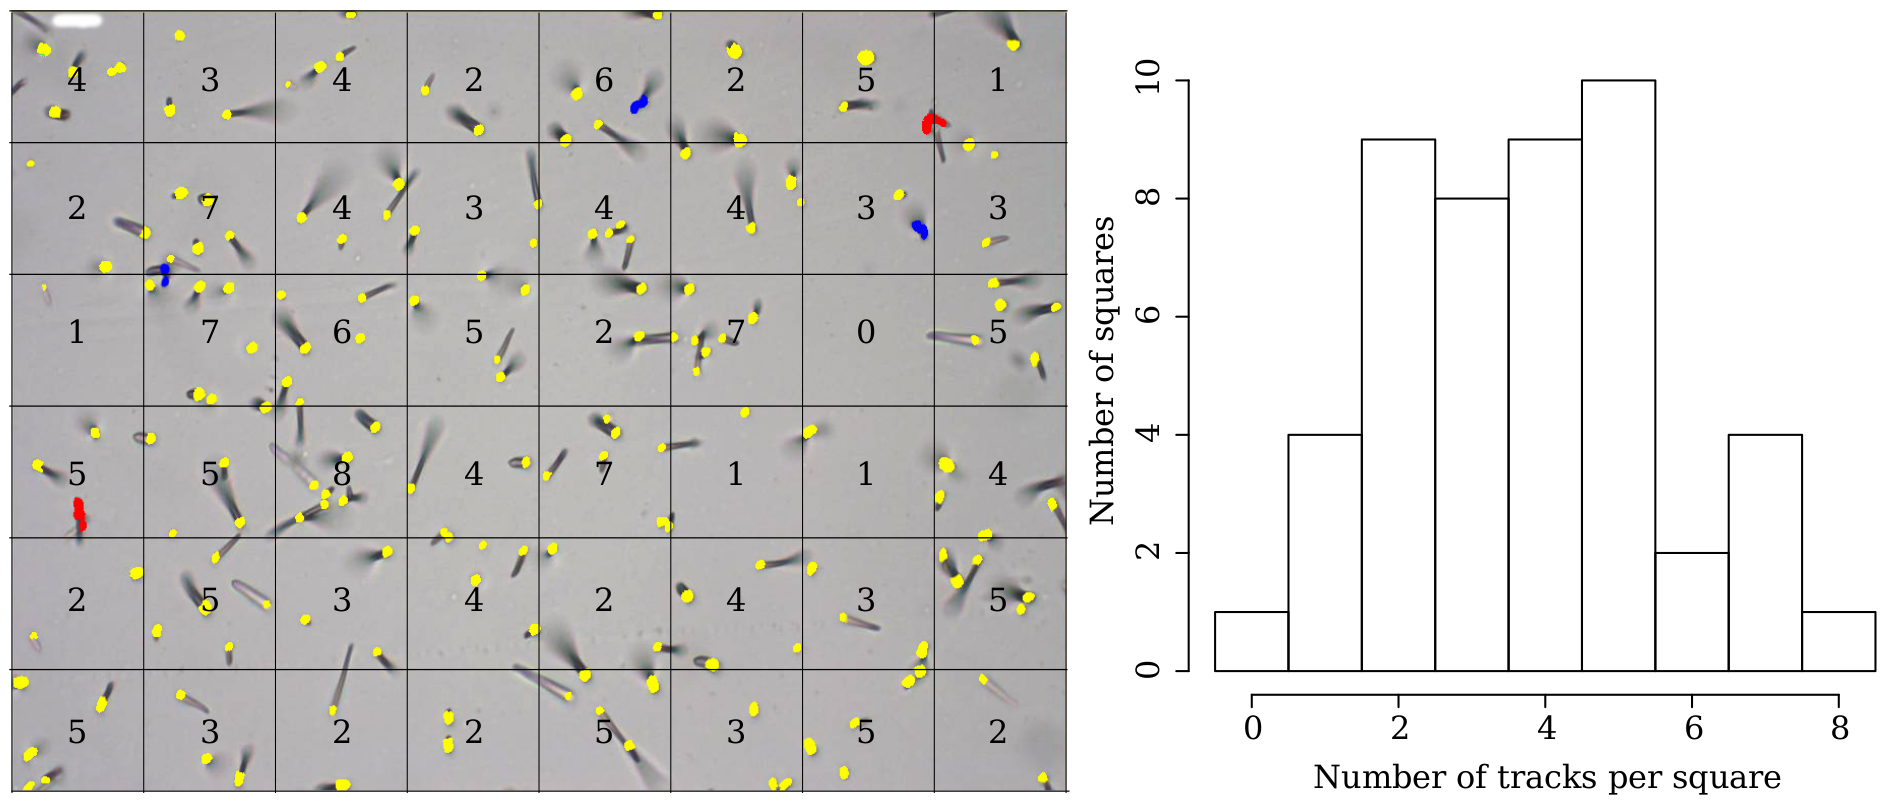
\includegraphics[width=\textwidth]{Poisson.png}
\caption{Left: induced fission tracks recorded in a mica detector
  attached to a dosimeter glass. Numbers indicate the number of tracks
  counted in 48 150$\times$150 $\mu m$-sized areas. Colours indicate
  single (yellow), double (blue) and triple (red) etch pits. Dosimeter
  glasses exhibit a uniform U-concentration so that the observed
  variation in the number of tracks is only due to Poisson
  statistics. Fission tracks were counted with FastTracks image
  recognition software \citep[see Chap.~4][]{gleadow2018}. Right: the
  frequency distribution of the FT counts, which has a mean of 3.7 and
  a variance of 3.5 counts per graticule, consistent with a Poisson
  distribution.}
\label{fig:Poisson}
\end{figure}

\section{Fission track plots}
\label{sec:visualisation}

The single grain uncertainties given by Eq. \ref{eq:shatt2} tend to be
very large.  For example, a grain containing just 4 spontaneous
fission tracks (i.e., N$_s$=4) is associated with an analytical
uncertainty of $\sqrt{4}$/4=50\% even ignoring the analytical
uncertainty associated with the $\zeta$-calibration constant, the
dosimeter glass, or the induced FT count.  The single grain age
precision of the FT method, then, is orders of magnitude lower than
that of other established geochronometers such as $^{40}$Ar/$^{39}$Ar
or $^{206}$Pb/$^{238}$U, which achieve percent or permil level
uncertainties. To overcome this limitation and `beat down the noise',
it is important that multiple grains are analysed from a sample and
averaged using methods described in
Sect.~\ref{sec:summarystats}. Multi-grain assemblages of FT data are
also very useful for sedimentary provenance analysis and form the
basis of a new field of research called `detrital thermochronology'
\citep{bernet2018, carter2018}.  Irrespective of the application, it
is useful for any multi-grain FT dataset to first be assessed
visually.  This Section will introduce three graphical devices to do
this: cumulative age distributions, (kernel) density estimates and
radial plots. To illustrate these graphical devices as well as the
different summary statistics of Sect.~\ref{sec:summarystats}, consider
the four different geological scenarios shown in Fig.~\ref{fig:ABCD}:

\begin{enumerate}[label=\Alph*.]
\item A rapidly cooled volcanic rock extruded at 15 Ma.
\item A slowly cooled intrusive rock exhibiting a range of Cl/F ratios
  resulting in a 150 Ma $\pm$ 20\% range of apparent FT ages.
\item A detrital sample collected from a river draining two volcanic
  layers extruded at 15 and 75 Ma, respectively.
\item A detrital sample collected from a river draining lithologies A
  and B.
\end{enumerate}

\subsection{The Cumulative Age Distribution (CAD)}

The cumulative distribution function cdf(x) describes the fraction of
the detrital age population whose age is less than or equal to x:

\begin{equation}
cdf(x) = P(t \leq x)
\end{equation}

Under Scenario I, the cdf consists of a simple step function,
indicating that 0\% of the grains are younger, and 100\% are older
than the extrusive age (Fig.~\ref{fig:ABCD}.I-a).  Under Scenario II,
the cdf is spread out over a wider range, so that 90\% of the ages are
between 90 and 210 Ma (Fig.~\ref{fig:ABCD}.II-a). Under Scenario III
(Fig.~\ref{fig:ABCD}.III-a), the cdf consists of two discrete steps at
15 and 75 Ma, the relative heights of which depend on the hypsometry
of the river catchment and the spatial distribution of erosion
\citep{vermeesch2007a}.  Finally, under Scenario IV, the cdf consists
of a discrete step from 0 to 50\% at 15 Ma, followed by a sigmoidal
rise to 100\% at 75Ma (Fig.~\ref{fig:ABCD}.IV-a).\\

In reality, the cdfs of Scenarios I-IV are, of course, unknown and
must be estimated from sample data, by means of an empirical
cumulative distribution function (ecdf), which may be referred to as a
Cumulative Age Distribution (CAD) in a geochronological context
\citep{vermeesch2007a}. A CAD is simply a step function in which the
single grain ages ($\hat{t}_j$, for j=1$\rightarrow$n) are plotted
against their rank order:

\begin{equation}
CAD(x) = \sum_{j=1}^{n} 1(\hat{t}_j \leq x)/n
\end{equation}

where 1(TRUE) = 1 and 1(FALSE) = 0. In contrast with the true cdfs,
the measured CADs are invariably smoother, as the analytical
uncertainties spread the ages out over a greater range. Because the
uncertainties of FT ages are so large, the difference between the
measured CADs and the true cdfs is very significant. Sections
\ref{sec:summarystats} and \ref{sec:mixtures} of this Chapter present
several algorithms to extract the key parameters of the true age
distribution (i.e, the cdfs) from the measurement distribution (CADs).

%\begin{landscape}
\begin{figure}
\centering
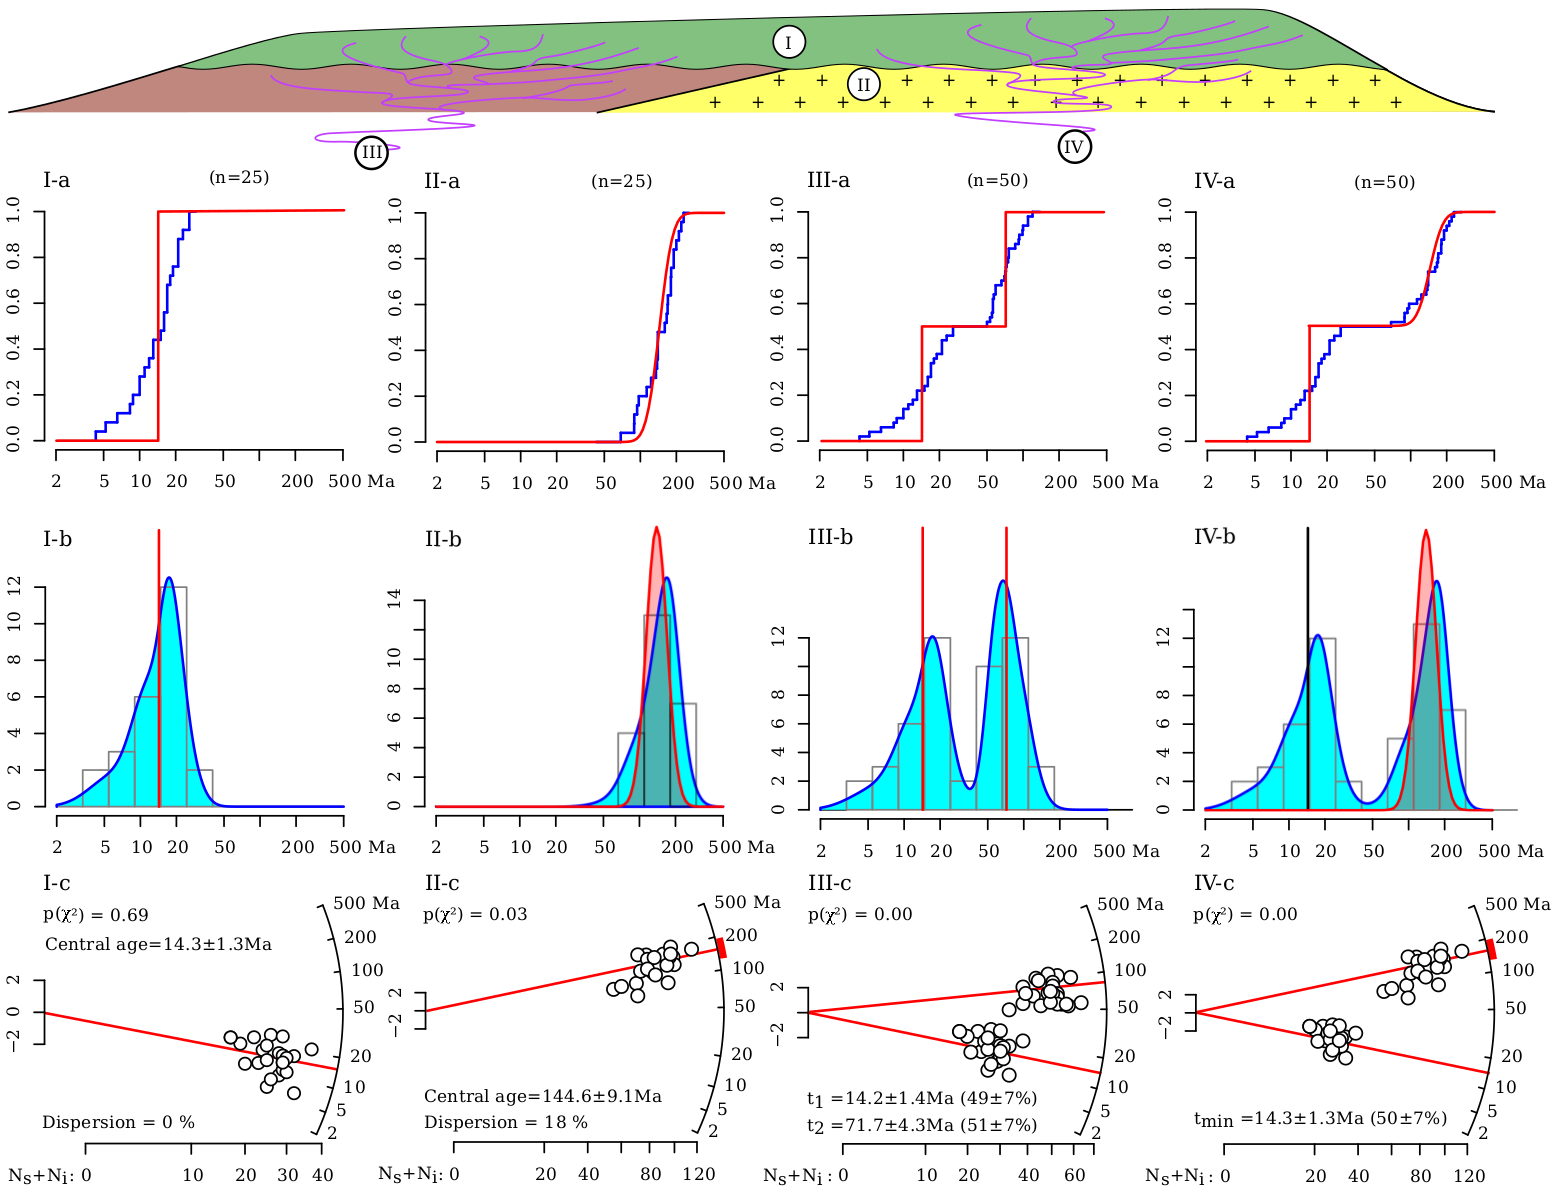
\includegraphics[width=\textwidth]{ABCD2.png}
\caption{Hypothetical landscape (hill) featuring four different
  sampling locations: I -- a rapidly cooled volcanic rock extruded at
  15 Ma; II -- a slowly cooled plutonic rock containing 150 Ma $\pm$
  20\% apatites; III -- a modern river draining lithology I and an
  older (75 Ma) volcanic deposit; and IV -- a second river draining
  lithologies I and II. For each of these scenarios, synthetic data
  were generated and plotted on three different graphical devices: a
  -- theoretical cumulative distribution function (cdf, red) and
  synthetic Cumulative Age Distribution (CAD, blue) of the samples at
  the four sampling locations; b -- theoretical pdfs (red) and
  synthetic sample Kernel Density Estimates (KDEs, blue) for the same
  synthetic data; c -- radial plots of the synthetic data with model
  fits (Sects. \ref{sec:summarystats} and \ref{sec:mixtures}).}
\label{fig:ABCD}
\end{figure}
%\end{landscape}

\subsection{(Kernel) Density Estimates (KDEs)}

The probability density function (pdf) is defined as the first
derivative of the cdf:

\begin{equation}
pdf(x) = \left.\frac{d[cdf(y)]}{d y}\right\vert_{x} \Leftrightarrow
cdf(x) = \int_{-\infty}^{x}pdf(y) dy
\end{equation}

Under Scenario I, the pdf is a discrete peak of zero width and
infinite height, marking the timing of the volcanic eruption
(Fig.~\ref{fig:ABCD}.I-b). In contrast, under Scenario II, the pdf is
a smooth (a)symmetric bell curve reflecting the spread in closing
temperatures and, hence, ages, associated with the range of
Cl/F-ratios present in apatites of this slowly cooled pluton
(Fig.~\ref{fig:ABCD}.II-b). Under Scenario III, the pdf consists of
two discrete spikes corresponding to the two volcanic events
(Fig.~\ref{fig:ABCD}.III-b). Finally, under Scenario IV, the pdf
effectively combines those of Scenarios I and II
(Fig.~\ref{fig:ABCD}.IV-b). The pdfs, like the cdfs discussed before,
are unknown but can be estimated from sample data. There are several
ways to do this.  Arguably the simplest of these is the histogram, in
which the observations are grouped into a number of discrete
bins. Kernel Density Estimates (KDEs) are a continuous alternative to
the histogram, which are constructed by arranging the measurements
from young to old along the time axis, adding a Gaussian `bell curve'
(or any other symmetric shape) on top of them, and then summing those
to create one continuous curve \citep{silverman1986,
  vermeesch2012b}. The standard deviation of the Gaussian `kernel' is
called the `bandwidth' of the estimator and may be chosen through a
host of different approaches, a proper discussion of which falls
outside the scope of this review \citep{abramson1982, silverman1986,
  botev2010, vermeesch2012b}. An important feature of all these
algorithms is that the bandwidth monotically decreases with increasing
sample size. Please note that the so-called `Probability Density Plot'
(PDP, not to be confused with pdf!), in which the analytical
uncertainty \citep[or 0.6 times the analytical
  uncertainty,][]{brandon1996} is used as a `bandwidth' does not
possess this feature. Therefore PDPs are not proper density estimates
and consequently their use is not recommended \citep{galbraith1998,
  vermeesch2012b}. Like the CAD, which is a smooth version of the cdf,
KDEs (and histograms) are smooth versions of the pdf. But whereas the
CAD has only been smoothed once, histograms and KDEs are smoothed
twice, once by the analytical uncertainties, and once by the width of
the bins or kernels. Because the analytical uncertainties of FT data
are so big, the components of FT age distributions are often spread
out very widely, resulting in poorly resolved KDEs (blue curves in
Figs.~\ref{fig:ABCD}.b).

\subsection{Radial plots}

Single grain fission track age uncertainties are not only very large,
they generally are also variable (`heteroscedastic'). Due to a
combination of Poisson sampling statistics and variable
U-concentrations, the analytical uncertainties propagated using
Eq. \ref{eq:shatt2} may vary over an order of magnitude within the
same sample. Neither CADs nor KDEs (let alone PDPs) are able to
capture this uncertainty.  The radial plot is a graphical device that
was specifically designed to address this issue
\citep{galbraith1988,galbraith1990a,dunkl2002,vermeesch2009c}. Given
j=1...n numerical values z$_j$ and their analytical uncertainties
$\sigma_j$, the radial plot is a bivariate ($x_j$,y$_j$) scatterplot
setting out a standardised estimate (y$_j$ = $(z_j-z_\circ)/\sigma_j$,
where z$_\circ$ is some reference value) against the single grain
precision (x$_j$ = 1/$\sigma_j$).  For FT data using the
EDM\footnote{The remainder of this and the next three Sections of this
  Chapter will focus on the EDM.  Alternative equations for ICP-MS
  based fission track data are provided in Sect.~\ref{sec:ICP}.}, it
is convenient to use the following definitions for z$_j$ and
$\sigma_j$ \citep{galbraith1990a}:

\begin{equation}
z_j = \arcsin\sqrt{\frac{N_{sj} + 3/8}{N_{sj}+N_{ij}+3/4}}
\label{eq:zj}
\end{equation}

and

\begin{equation}
\sigma_j = \frac{1}{2\sqrt{N_{sj}+N_{ij}+1/2}}
\label{eq:sj}
\end{equation}

Thus, precise measurements plot towards the right-hand side of the
radial plot whilst imprecise measurements plot closer to the origin.
A single grain age may be read off by extrapolating a line from the
origin (0,0) of the radial plot through the sample point (x$_j$,y$_j$)
to a radial scale plotted at some convenient distance.  Similarly, the
analytical uncertainty can be obtained by extrapolating lines from the
origin to the radial scale through the top and the bottom of an
imaginary 2$\sigma$-error bar added to each sample point.  Finally,
drawing two parallel lines at 2$\sigma$ distances from either side of
the origin allow the analyst to visually assess whether all the single
grain ages within a sample agree within the analytical
uncertainties.\\

Revisiting Scenario I of Fig.~\ref{fig:ABCD}, the data points plot
within a 2$\sigma$ band on the radial plot, consistent with a single
discrete age component (Fig.~\ref{fig:ABCD}.I-c). Under Scenario II,
the data are more dispersed and scatter beyond the 2$\sigma$ band,
reflecting the dispersion of the underlying geological ages
(Fig.~\ref{fig:ABCD}.II-c). Under Scenario III, the data are randomly
scattered along two linear trajectories which represent the two
volcanic events (Fig.~\ref{fig:ABCD}.III-c). Finally, Scenario IV
combines the radial patterns of Scenarios I and II, as expected
(Fig.~\ref{fig:ABCD}.IV-c). Of all the summary plots in
Fig.~\ref{fig:ABCD}, the radial plot contains the largest amount of
quantitative information about the age measurements and about the
underlying geological ages. Using the graphical design principles of
\citet{tufte1983}, the radial plot exhibits a far higher
`ink-to-information ratio' than the CAD, KDE or histogram.  We will
therefore use it as a basis from which to introduce the summary
statistics discussed in the next Section of this Chapter.

\section{Summary statistics}
\label{sec:summarystats}

The previous Sections have shown that the presence of large and highly
variable analytical uncertainties can easily obscure the underlying
age distribution and all the geologically meaningful information
encoded by it. The next two Sections will introduce some useful
summary statistics which can be used to disentangle that geologically
meaningful information from the random noise produced by the Poisson
counting uncertainties.

\subsection{The pooled age}
\label{sec:pooled}

Let us begin with the single discrete age component in Scenario I of
the previous Section.  Several approaches can be used to estimate this
age from a set of noisy sample data. Panels I-a, I-b and I-c of
Fig.~\ref{fig:ABCD} show that the single grain age estimates follow an
asymmetric probability distribution (symmetric when plotted on a
logarithmic scale) which is skewed toward older ages. This is a
consequence of the fact that, if $N_{sj}$ and $N_{ij}$ are sampled
from two independent Poisson distributions with expected values
$\rho_s$ and $\rho_i$, respectively, then the conditional probability
of $N_{sj}$ on $N_{sj} + N_{ij}$ follows a Binomial distribution:

\begin{equation}
P(N_{sj}|N_{sj}+N_{ij}) = {{N_{sj}+N_{ij}}\choose{N_{sj}}}
\theta^{N_{sj}} (1-\theta)^{N_{ij}} \equiv f_j(\theta)
\label{eq:pbinom}
\end{equation}

where $\theta \equiv \rho_s/(\rho_s+\rho_i)$ and ${a}\choose{b}$ is
the Binomial coefficient. Given a sample of n sets of FT counts, this
leads to the following (log-)likelihood function for $\theta$:

\begin{equation}
\mathcal{L}(\theta) = \sum\limits_{j=1}^{n} \ln f_j(\theta)
\label{eq:Lpooled}
\end{equation}

where $f_j(\theta)$ is the probability mass function for the j$^{th}$
grain defined in Eq. \ref{eq:pbinom}. As a first approach to obtaining
an `average' age, one might be tempted to simply take the arithmetic
mean of the single grain age estimates. Unfortunately, the arithmetic
mean does not cope well with outliers and asymmetric distributions and
therefore yields poor estimates of the geological age. The geometric
mean fares much better. It is closely related to the `central age',
which is discussed in Sect.~\ref{sec:randomeffects}. The `pooled age'
is obtained by maximising Eq. \ref{eq:Lpooled} to obtain a `maximum
likelihood' estimate ($\hat{\theta}$), and substituting
$e^{\hat{\theta}}$ for $N_s/N_i$ in Eq. \ref{eq:tzeta}, where $N_s =
\sum_{j=1}^{n} N_{sj}$ and $N_i = \sum_{j=1}^{n} N_{ij}$. This is
equivalent to taking the sum of all the spontaneous and induced
tracks, respectively, and treating these as if they belonged to a
single crystal.  This procedure yields the correct age if the true
ages are indeed derived from a single discrete age component (i.e.,
Scenario I). However, if there is any dispersion of the true FT ages,
as is the case under Scenario II, then the pooled age will be biased
towards values that are far too old. Whether this is the case or not
can be verified using a formalised statistical hypothesis
test. \citet[][p.46]{galbraith2005} shows that in the absence of
excess dispersion, the following statistic:

\begin{equation}
  c^2 = \frac{1}{N_sN_i}\sum\limits_{j=1}^{n}\frac{(N_{sj}N_i-N_{ij}N_s)^2}{N_{sj}+N_{ij}}
  \label{eq:X2}
\end{equation}

follows a Chi-square distribution with n-1 degrees of freedom. The
probability of observing a value greater than $c^2$ under this
distribution is called the p-value and can be used to formally test
the assumption of zero dispersion. A cutoff of 0.05 is often used as a
criterion to abandon the single grain age model of Scenario I and,
hence, the pooled age.

\subsection{Central ages and `overdispersion'}
\label{sec:randomeffects}

A more meaningful estimate for Scenario II is obtained using a
two-parameter `random effects' model, in which the true
$\rho_s/\rho_i$-ratio is assumed to follow a log-normal distribution
with location parameter $\mu$ and scale parameter $\sigma$
\citep{galbraith1993}:

\begin{equation}
\ln (\rho_s/\rho_i) \sim \mathcal{N}(\mu,\sigma^2)
\label{eq:logrhosrhoi}
\end{equation}

This model gives rise to a two-parameter log-likelihood function:

\begin{equation}
  \mathcal{L}(\mu,\sigma^2) = \sum\limits_{j=1}^{n}
  \ln f_j(\mu,\sigma^2)
\label{eq:Lcentral}
\end{equation}

where the probability mass function $f_j(\mu,\sigma^2)$ is defined as:

\begin{equation}
  f_j(\mu,\sigma^2) = {{N_{sj}+N_{ij}}\choose{N_{sj}}}
  \int\limits_{-\infty}^{\infty} \frac{e^{\beta N_{sj}} \left( 1 +
    e^\beta \right)^{-N_{sj}-N_{ij}}} {\sigma\sqrt{2\pi}
    e^{(\beta-\mu)^2/(2\sigma^2)}} d\beta
  \label{eq:fjms}
\end{equation}

in which the FT ratios are subject to two sources of variation: the
Poisson uncertainty described by Eq.  \ref{eq:Lpooled} and an
`(over)dispersion' factor $\sigma$.  Maximising Eq. \ref{eq:Lcentral}
results in two estimates $\hat{\mu}$ and $\hat{\sigma}$ and their
respective standard errors.  Substituting $e^{\hat{\mu}}$ for
$N_s/N_i$ in Eq. \ref{eq:tzeta} produces the so-called `central
age'. $\hat{\sigma}$ estimates the overdispersion, and quantifies the
excess scatter of the single grain ages which cannot be explained by
the Poisson counting statistics alone. This dispersion can be just as
informative as the central age itself, as it encodes geologically
meaningful information about the compositional heterogeneity and
cooling history of the sample.  In the absence of excess dispersion,
i.e. if $\hat{\sigma}$=0, the central age equals the pooled age, so
there is not really any reason to use the pooled age at all.

\section{Mixture models}
\label{sec:mixtures}

A FT dataset may fail the Chi-square test introduced in the previous
Section for different reasons. The true ages may exhibit excess
scatter according to Eq. \ref{eq:Lcentral}. Or it may be so that there
are more than one age component \citep{galbraith1990b, galbraith1993}.
These components could either be discrete age peaks (Scenario III), or
they could be any combination of discrete and continuous age
components (Scenario IV).

\subsection{Finite mixtures}
\label{sec:finite}

Finite mixture models are a generalisation of the discrete age model
of Scenario I in which the true ages are not derived from a single,
but from multiple age populations \citep{galbraith1990b}. Scenario III
is an example of this with two such components.  In contrast with the
common age model of Scenario I, which is completely described by a
single parameter ($\theta$, or the pooled age), and the random effects
model, which comprises two parameters ($\mu$ and $\sigma$, or the
central age and overdispersion), the finite mixture of Scenario III
requires three parameters. These are the age of the first component,
the age of the second component, and the proportion of the grains
belonging to the first component. The proportion belonging to the
second component is simply the complement of the latter
value. Generalising to N components, the log-likelihood function
becomes:

\begin{equation}
\mathcal{L}(\pi_{k},\theta_{k}, k = 1 \ldots N) = 
\sum\limits_{j=1}^{n} \ln \left[
\sum\limits_{k=1}^{N} \pi_k f_j(\theta_k)
\right]
\mbox{~with~} \pi_N = 1-\sum\limits_{k=1}^{N-1}\pi_k
\label{eq:Lfinite}
\end{equation}

where $f_j(\theta_k)$ is given by Eq. \ref{eq:pbinom}.  Eq.
\ref{eq:Lfinite} can be solved numerically. Applying it to the single
component dataset of Scenario I again yields the pooled age as a
special case. The detrital FT ages in Scenario III clearly fall into
two groups so it is quite evident that there are two age
components. Unfortunately the situation is not always this clear. Due
to the large single grain age uncertainties discussed in
Sect.~\ref{sec:EDM}, the boundaries between adjacent age components
are often blurred, making it difficult to decide how many `peaks' to
fit. Several statistical approaches may be used to answer this
question.  One possibility is to use a log-likelihood ratio
test. Suppose that we have solved Eq. \ref{eq:Lfinite} for the case of
N=2 age components, and denote the corresponding maximum log-likelhood
value as $\mathcal{L}_2$. We then consider an alternative model with
N=3 components.  This results in two additional parameters ($\pi_2$
and $\theta_3$) and a new maximum log-likelihood value,
$\mathcal{L}_3$. We can assess whether the three component model is a
significant improvement over the two component fit by comparing twice
the difference between $\mathcal{L}_3$ and $\mathcal{L}_2$ to a
Chi-square distribution with two degrees of freedom (because we have
added two additional parameters) and calculating the corresponding
p-value like before. An illustration of the log-likelihood ratio test
is provided in Sect.~\ref{sec:continuous}.  An alternative approach is
to maximise the so-called Bayes Information Criterion (BIC), which is
defined as

\begin{equation}
BIC = -2 \mathcal{L}_{max} + p ~ \ln (n)
\end{equation}

where $\mathcal{L}_{max}$ is the maximum log-likelihood of a model
comprising p parameters and n grains. A worked example of this method
is omitted for brevity and the reader is referred to
\citet[][p.91]{galbraith2005} for further details.

\subsection{Continuous mixtures}
\label{sec:continuous}

So far we have considered pdfs consisting of a single discrete age
peak (Scenario I), a single continuous age distribution (Scenario II)
and multiple discrete age peaks (Scenario III).  The logical next step
is to consider multiple continuous age distributions
\citep{jasra2006}.  In principle such models can be obtained by
maximising the following likelihood function

\begin{equation}
\mathcal{L}(\pi_{k},\mu_{k},\sigma^2_{k}, k = 1 \ldots N) = 
\sum\limits_{j=1}^{n} \ln \left[
\sum\limits_{k=1}^{N} \pi_k f_j(\mu_k,\sigma^2_k) 
\right]
\mbox{~with~} \pi_N = 1-\sum\limits_{k=1}^{N-1}\pi_k
\label{eq:Lcontmix}
\end{equation}

where $f_j(\mu_k,\sigma_k^2)$ is given by Eq.~\ref{eq:fjms}. However,
in reality this is often impractical due to the high number of
parameters involved, which require exceedingly large datasets. In
detrital geochronology, the analyst rarely knows that the data are
underlain by a continuous mixture and so it is tempting to reduce the
number of unknown parameters by simply assuming a discrete
mixture. Unfortunately, this is fraught with problems as well since
there is no upper bound on the number of discrete age components to
fit to a continuous dataset. To illustrate this point, let us
reconsider the dataset of Scenario II, this time applying a finite
mixture model rather than the random effects model of
Sect.~\ref{sec:randomeffects}.  For a small sample of n=10 grains, the
Chi-square test for age homogeneity yields a p-value of 0.47, which is
above the 0.05 cutoff and thus provides insufficient evidence to
reject the common age model (Table~\ref{tab:Lratio} and
Fig.~\ref{fig:mixtures}.a).  Increasing the sample size to n=25
results in a p-value of 0.03, justifying the addition of additional
model parameters (Fig.~\ref{fig:ABCD}.I-c). Further increasing the
sample size to n=100 reduces the likelihood of the common age model
(Eq.~\ref{eq:Lpooled}) and results in a p-value of 0.0027, well below
the 0.05 cutoff. Let us now replace the common age model with a two
component finite mixture model. For the same 100-grain sample, this
increases the log-likelihood from -4598.3 to -4591.4
(Table~\ref{tab:Lratio}). Using the log-likelihood ratio test
introduced in Sect.~\ref{sec:finite}, that corresponds to a Chi-square
value of 2 $\times$ (4598.3 - 4591.4) = 13.8 and a p-value of 0.001,
lending support to the abandonment of the single age model in favour
of the two parameter model (Fig.~\ref{fig:mixtures}.b).  However,
doing the same calculation for a three component model yields a
log-likelihood of -4590.6 and a Chi-square value of 2 $\times$ (4591.4
- 4590.6) = 1.6, resulting in an insignificant p-value of 0.45
(Table~\ref{tab:Lratio}). Thus, the 100-grain sample does \emph{not}
support the three component model. It is only when the sample size is
increased from 100 to 1000 grains that the Chi-square test gains
enough `power' to justify the three component finite mixture model
(Fig.~\ref{fig:mixtures}.c). It is easy to see that this trend
continues \emph{ad infinitum}: with increasing sample size, it is
possible to add ever larger numbers of components
(Fig.~\ref{fig:mixtures}).\\

One might object to this hypothetical example by noting that the
finite mixture model is clearly inappropriate for a dataset that is
derived from a continuous mixture.  But the key point is that
\emph{all} statistical models are inappropriate to some degree.  Even
the random effects model is a mathematical abstraction which does not
exist in the real world. True age distributions (pdfs) may be
approximately (log)normal as in Scenario I, but they are never exactly
so. Given a sufficiently large sample, formalised statistical
hypothesis tests such as Chi-square are always able to detect even the
most minute deviation from any hypothetical age model and thereby
provide statistical justification to add further parameters.  This is
important in the common situation where one is interested in the
youngest age component of a fission track age distribution, for
example when one aims to calculate `lag times' and estimate exhumation
rates \citep{garver1999,bernet2018}. It would be imprudent to estimate
the lag-time by applying a general purpose multi-component mixture
model and simply picking the youngest age component. This would
provide a biased estimate of the minimum age, which would steadily
drift towards younger values with increasing sample size
(Fig.~\ref{fig:mixtures}).  Instead, it is better to use a simpler but
more stable and robust model employing
three\footnote{Eq.~\ref{eq:Lminagemod} may be simplified by imposing
  the requirement that $\mu=e^{\theta}$, which significantly benefits
  numerical stability, while having only a minor effect on the
  accuracy of $\theta$.}  or four parameters to explicitly determine
the minimum age component:

\begin{equation}
  \mathcal{L}(\pi,\theta,\mu,\sigma^2) =
  \sum\limits_{j=1}^{n} \ln \left[
    \pi f_j(\theta) + (1-\pi) f'_j(\mu,\sigma^2)
    \right]
\label{eq:Lminagemod}
\end{equation}

where $f_j(\theta)$ is given by Eq.~\ref{eq:pbinom} and
$f'_j(\mu,\sigma^2)$ is a truncated version of Eq.~\ref{eq:fjms}
\citep{galbraith1993}. Applying this model to the synthetic example of
Scenario IV correctly yields the age of the youngest volcanic unit
regardless of sample size (Fig.~\ref{fig:ABCD}.IV-c). In conclusion,
statistical hypothesis tests such as Chi-square can be used to prevent
overinterpreting perceived `clusters' of data which may arise from
random statistical sampling fluctuations. But they must be used with
caution, bearing in mind the simplifying assumptions which all
mathematical models inevitably make, and the dependence of test
statistics and p-values on sample size.  Ignoring this dependence may
lead to statistical models which might make sense in a mathematical
sense, but have little or no geological relevance. This note of
caution applies not only to mixture modelling but even more so to
thermal history modelling, as will be discussed next.

\begin{table}
\centering
\begin{tabular}{r|ccccccc}
       & $\mathcal{L}_1$  & p($\chi^2_2$) & $\mathcal{L}_2$  &  p($\chi^2_2$) & 
         $\mathcal{L}_3$ & p($\chi^2_2$) & $\mathcal{L}_4$   \\
n=10   & -422.4   & 0.67 & -422.0   & 1.00 & -422.0   & 1.00 & -422.0 \\
n=100  & -4598.3  & 0.001 & -4591.4  & 0.45 & -4590.6  & 1.00 & -4590.6 \\
n=1000 & -45030.7 & 0.00 & -44966.5 & 0.00003 & -44956.1 & 0.67 & -44955.7 \\
\end{tabular}
\caption{Application of the log-likelihood ratio test to a finite
  mixture fitting experiment shown in Fig.~\ref{fig:mixtures}. Rows
  mark different sample sizes (with n marking the number of grains)
  drawn from Scenario II. Columns labeled as $\mathcal{L}_N$ show the
  log-likelihood of different model fits, where N marks the number of
  components. Columns labeled as p($\chi^2_2$) list the p-values of a
  Chi-square test with two degrees of freedom, which can (but in this
  case should not) be used to assess whether it is statistically
  justified to increment the number of fitting parameters (N) by one.}
\label{tab:Lratio}
\end{table}

\begin{figure}[!ht]
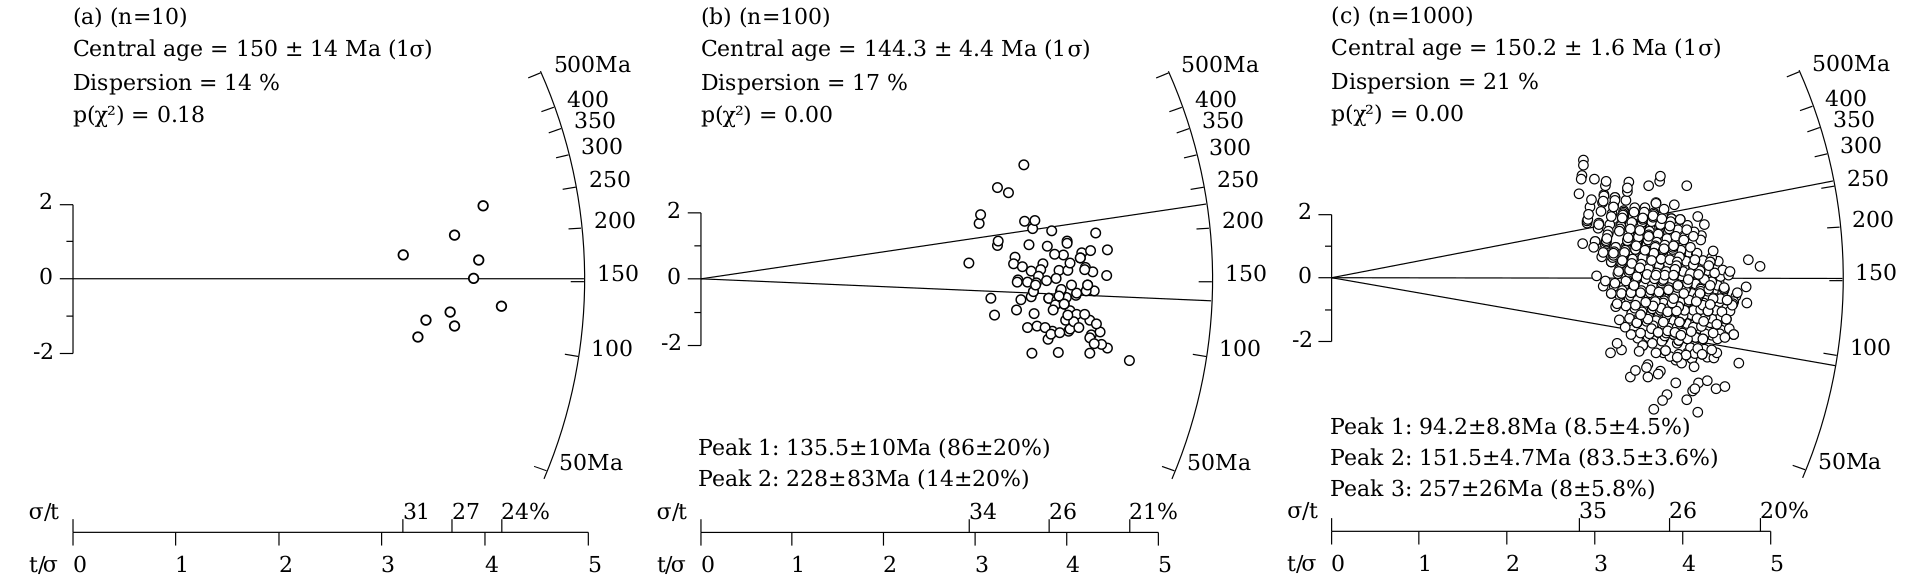
\includegraphics[width=\textwidth]{mixtures.png}
\caption{Application of finite mixture modelling to the continuous
  mixture of Scenario II (Fig.~\ref{fig:ABCD}). Increasing sample size
  from left (a) to right (c) provides statistical justification to fit
  more components using the log-likelihood ratio approach of
  Table~\ref{tab:Lratio}.  Note that the age of the youngest age
  component gets progressively younger with increasing sample size,
  from 150 Ma for sample (a) to 94 Ma for sample (c), and is therefore
  not a reliable estimator of the minimum age. p($\chi^2$) marks the
  p-value of the Chi-square test for age homogeneity and \emph{not}
  the log-likelihood ratio tests of Table~\ref{tab:Lratio}.}
\label{fig:mixtures}
\end{figure}

\section{Inverse modelling}
\label{sec:modelling}

So far in this Chapter we have made the implicit assumption (in
Eq.~\ref{eq:tzeta}) that all fission tracks have the same
length. In reality, however, this is not the case, and the length of
(apatite) fission tracks varies anywhere between 0 and 16$\mu m$ as a
function of the thermal history and chemical composition of a sample
\citep{gleadow1986}. If the compositional effects \citep[notably the
  Cl/F ratio,][]{green1986} are well characterised, then the measured
length distribution of horizontally confined fission tracks can be
used to reconstruct the thermal history of a sample. Laboratory
experiments show that the thermal annealing of fission tracks in
apatite obeys a so-called `fanning Arrhenius' relationship, in which
the degree of shortening logarithmically depends on both the amount
and duration of heating \citep{green1985, laslett1987, laslett1996,
  ketcham1999, ketcham2007}:

\begin{equation}
\ln \left(1 - \sqrt[\Lambda]{L/L_\circ}\right) = 
c_0 - c_1 \frac{\ln (t) - \ln (t_c)}{1/T - 1/T_c}
\end{equation}

where $L_\circ$ and $L$ are the initial and measured track length, t
and T are time and absolute temperature, respectively, and c$_0$,
c$_1$, $\Lambda$, t$_c$ and T$_c$ are fitting parameters
\citep{laslett1996, ketcham1999}. Using these laboratory results,
thermal history reconstructions are a two-step process. First, a large
number of random thermal histories are generated, and for each of
these the fanning Arrhenius relationship is used to predict the
corresponding FT length distribution \citep{corrigan1991, lutz1991,
  gallagher1995, willett1997, ketcham2000, ketcham2005,
  gallagher2012}. Then, these `forward model' predictions are compared
with the measured values and the `best' matches are retained for
geological interpretation. All the `inverse modelling' software that
has been developed over the years for the purpose of thermal history
reconstructions essentially follows this same recipe. The most
important difference between these algorithms is how they assess the
goodness of fit and decide which candidate t-T paths to retain and
which to reject.  One class of software, including the popular HeFTy
program and its predecessor AFTSolve \citep{ketcham2000,ketcham2005},
use the p-value of formalised hypothesis tests like the Chi-square
test described in the previous Sections, to decide whether the
measured FT length distribution is a `good' (p$>$0.5), `acceptable'
(0.5$>$p$>$0.05) or `poor' (p$<$0.05) fit. The problem with this
approach is that, due to the dependence of p-values on sample size, it
inevitably breaks down for large datasets. This is because the
statistical `power' of statistical hypothesis test to resolve even the
tiniest disagreement between the measured and the predicted length
distribution, monotonically increases with increasing sample size
\citep{vermeesch2014}.\\

A second class of inverse modelling algorithms \citep[including
  QTQt,][]{gallagher2012} does not employ formalised hypothesis tests
or p-values, but aims to extract the `most likely' thermal history
models among all possible t-T paths \citep{gallagher1995,
  willett1997}. These methods do not `break down' when they are
applied to large datasets. On the contrary, large datasets are
`rewarded' in the form of tighter `credibility intervals' and higher
resolution t-T paths. Furthermore, they are easily extended to
multi-sample and multi-method datasets. However, with great power also
comes great responsibility. \citet{vermeesch2014} show that QTQt
always produces a `best fitting' thermal history even for physically
impossible datasets. To avoid this potential problem, it is of
paramount importance that the model predictions are shown alongside
the FT data \citep{gallagher2012, gallagher2016, vermeesch2014}.

\section{LA-ICP-MS based FT dating}
\label{sec:ICP}

The EDM outlined in Sect.~\ref{sec:EDM} continues to be the most
widely used analytical protocol in FT dating. However, over the past
decade, an increasing number of laboratories have abandoned it and
switched to LA-ICP-MS as a means of determining the uranium
concentration of datable minerals, thus reducing sample turnover time
and removing the need to handle radioactive materials
\citep{hasebe2004, hasebe2009, chew2012, soares2014, abdullin2016,
  vermeesch2017}. The statistical analysis of ICP-MS based FT data is
less straightforward and less well developed than that of the EDM. As
described in Sect.~\ref{sec:EDM}, the latter is based on simple ratios
of Poisson variables, and forms the basis of a large edifice of
statistical methods which cannot be directly applied to ICP-MS based
data. This Section provides an attempt to address this issue.

\subsection{Age equation}
\label{sec:ICPage}

The FT age equation for ICP-MS based data is based on
Eq.~\ref{eq:tFT}:

\begin{equation}
\hat{t} = \frac{1}{\lambda_D}
\ln \left(1 + \frac{\lambda_D}{\lambda_f}\frac{N_s}{[\hat{U}] A_s R ~ q}\right)
\label{eq:tICP}
\end{equation}

where $N_s$ is the number of spontaneous tracks counted over an area
$A_s$, q is an `efficiency factor' \citep[$\sim$0.93 for apatite and
  $\sim$1 for
  zircon,][]{iwano1998,enkelmann2003,jonckheere2003b,soares2013} and
$[\hat{U}]$ is the $^{238}$U-concentration (in atoms per unit volume)
measured by LA-ICP-MS. Eq. \ref{eq:tICP} requires an explicit value
for $\lambda_f$ and assumes that the etchable range (R) is accurately
known \citep{soares2014}. Alternatively, these factors may be folded
into a calibration factor akin to the EDM (Eq.~\ref{eq:tzetahat}):

\begin{equation}
\hat{t} = \frac{1}{\lambda_D}
\ln \left(1+\frac{1}{2}\lambda_D\hat{\zeta}\frac{N_s}{A_s[\hat{U}]}\right)
\label{eq:tzetahatICP}
\end{equation}

in which $\hat{\zeta}$ is determined by analysing a standard of known
FT age \citep{hasebe2004}. Note that, in contrast with the `absolute'
dating method of Eq.~\ref{eq:tICP}, the $\zeta$-calibration method of
Eq.~\ref{eq:tzetahatICP} allows $[\hat{U}]$ to be expressed in any
concentration units (e.g., ppm or wt\% of total U) or could even be
replaced with the measured U/Ca-, U/Si- or U/Zr-ratios produced by the
ICP-MS instrument. The standard error of the estimated age is given by

\begin{equation}
s[\hat{t}] \approx \hat{t} \sqrt{ 
  \left(\frac{s[\hat{\zeta}]}{\hat{\zeta}}\right)^2 +
  \left(\frac{s[\hat{U}]}{\hat{U}}\right)^2 +
  \frac{1}{N_s}
}
\label{eq:shatt4}
\end{equation}

for the $\zeta$-calibration approach (Eq.~\ref{eq:tzetahatICP}), where
$s[\hat{U}]$ is the standard error of the uranium concentration
measurement (or the U/Ca-ratio measurement, say), which can be
estimated using two alternative approaches as discussed in
Sect.~\ref{sec:uICPerr}. Eq.~\ref{eq:shatt4} can also be applied to
the `absolute' dating method (Eq.~\ref{eq:tICP}) by simply setting
$s[\hat{\zeta}]/\hat{\zeta}=0$.

\subsection{Error propagation of LA-ICP-MS based uranium concentrations}
\label{sec:uICPerr}

Uranium-bearing minerals such as apatite and zircon often exhibit
compositional zoning, which must either be removed or quantified in
order to ensure unbiased ages.

\begin{enumerate}
  \item The effect of compositional zoning can be \emph{removed} by
    covering the entire counting area with one large laser spot
    \citep{soares2014} or a raster \citep{hasebe2004}. $s[\hat{U}]$ is
    then simply given by the analytical uncertainty of the LA-ICP-MS
    instrument, which typically is an order of magnitude lower than
    the standard errors of induced track counts in the EDM.
\item Alternatively, the uranium-heterogeneity can be
  \emph{quantified} by analysing multiple spots per analysed grain
  \citep{hasebe2009}. In this case, it is commonly found that the
  variance of the different uranium-measurements within each grain far
  exceeds the formal analytical uncertainty of each spot
  measurement. The following paragraphs will outline a method to
  measure that dispersion, even if some of the grains in a sample were
  only visited by the laser once.
\end{enumerate}

The true statistical distribution of the U-concentrations within in
each grain is unknown but is likely to be log-normal:

\begin{equation}
\ln [\hat{U}_{jk}] \sim \mathcal{N}(\mu_j,\sigma_j^2)
\label{eq:lognorm}
\end{equation}

where $\hat{U}_{jk}$ is the k\textsuperscript{th} (out of $n_j$)
uranium concentration measurements, and $\mu_j$ and $\sigma_j^2$ are
the (unknown) mean and variance of a Normal
distribution. Unfortunately it is difficult to accurately estimate
these two parameters from just a handful of spot measurements, and it
is downright impossible if $n_j$ = 1. This problem requires a
simplifying assumption such as $\sigma_j$ = $\sigma$ $\forall$ j. In
that case we can estimate the parameters of Eq. \ref{eq:lognorm}
as follows:

\begin{equation}
\hat{\mu}_j = \sum\limits_{k=1}^{n_j} \ln [\hat{U}_{jk}]/n_j
\end{equation}

and

\begin{equation}
\hat{\sigma}^2 = \sum\limits_{j=1}^{n} \sum\limits_{k=1}^{n_j}
\left( \ln [\hat{U}_{jk}] - \hat{\mu}_j \right)^2 / 
\sum\limits_{j=1}^{n} (n_j - 1).
\end{equation}

The (geometric) mean uranium concentration and standard error of the
j\textsuperscript{th} grain are then given by

\begin{equation}
\hat{U}_j = \exp[\hat{\mu}_j]
\end{equation}

and

\begin{equation}
s[\hat{U}_j] = \hat{U}_j \hat{\sigma}
\end{equation}

which may be directly plugged into Eqs.~\ref{eq:tICP}-\ref{eq:shatt4}
to calculate FT ages and uncertainties. Note that this procedure
ignores the analytical uncertainty of the individual U-measurements. A
more sophisticated approach that combines the analytical uncertainties
of the U-measurements with the dispersion of multiple spot
measurements is provided by \citet{vermeesch2017}.

\subsection{Zero track counts}
\label{sec:zeroICP}

In contrast with the EDM, ICP-MS based FT data do not offer an easy
way to deal with zero track counts. One pragmatic solution to this
problem is to approximate the ICP-MS based uranium concentration
measurement with an `equivalent induced track density', using the
following linear transformation:

\begin{equation}
\hat{N}_{ij} = \rho_j A_{sj} [\hat{U}_j]
\end{equation}

where $A_{sj}$ is the area over which the spontaneous tracks of the
j$^{th}$ grain have been counted and $\rho_j$ plays a similar role as
$\rho_d$ in Eq.~\ref{eq:tzeta}. From the requirement that the variance
of a Poisson-distributed variable equals its mean
(Sect.~\ref{sec:EDM}), it follows that:

\begin{equation}
\hat{N}_{ij} = \rho_j^2 A_{sj}^2 s[\hat{U}_j]^2
\end{equation}

from which it is easy to determine $\rho_j$. The analytical uncertainty
for the j$^{th}$ single grain age is then given by:

\begin{equation}
  s[\hat{t}_j] \approx \hat{t}_j \sqrt{\frac{1}{N_{sj}} +
    \frac{1}{\hat{N}_{ij}} +
    \left(\frac{s[\hat{\zeta}]}{\zeta}\right)^2}
  \label{eq:shattPseudoZeta}
\end{equation}

where $N_{sj}$ indicates the number of spontaneous tracks measured in
the j$^{th}$ grain, and $s[\hat{\zeta}]/\zeta=0$ for the `absolute'
dating approach (Eq.~\ref{eq:tICP}). The zero track problem can then
be solved using the methods mentioned in Sect.~\ref{sec:EDM}.

\subsection{Plots and models}

To plot ICP-MS based fission track data on a radial plot, we can
replace Eqs.~\ref{eq:zj} and \ref{eq:sj} with

\begin{align}
  z_j & = \ln (\hat{t}_j) \mbox{,}   \label{eq:zj2} \\
  \mbox{and~} s_j & = \sqrt{ 
    \left(\frac{s[\hat{\zeta}]}{\hat{\zeta}}\right)^2 +
    \left(\frac{s[\hat{U}]}{\hat{U}}\right)^2 +
    \frac{1}{N_s}
  }   \label{eq:sj2}
\end{align}

respectively \citep{galbraith2010b}. Alternatively, a square root
transformation may be more appropriate for young and/or U-poor samples
(Galbraith, \textit{pers. commun.}):

\begin{align}
  z_j & = \sqrt{\hat{t}_j} \mbox{,}   \label{eq:zj3} \\
  \mbox{and~} s_j & = s[\hat{t}_j]\bigg/\left(2\sqrt{\hat{t}_j}\right)
  \label{eq:sj3}
\end{align}

The Binomial Likelihood function of
Sect.~\ref{sec:randomeffects} may be replaced with an alternative form
assuming Normal errors. Thus, Eq.~\ref{eq:Lpooled} becomes:

\begin{equation}
\mathcal{L}(\theta) = \sum\limits_{j=1}^{n}
\ln \left[ \mathcal{N}(z_j|\theta,\sigma_j^{\prime 2}) \right]
\label{eq:Lpoolednorm}
\end{equation}

where $\mathcal{N}(a|b,c)$ stands for ``the probability density of
observing a value \emph{a} from a Normal distribution with mean
\emph{b} and variance \emph{c}'', z$_j$ is defined by Eq.~\ref{eq:zj2}
and $\sigma'_j$ is given by

\begin{equation}
\sigma'_j = s[\hat{t}_j]/\hat{t}_j
\end{equation}

The Chi-square statistic (Eq.~\ref{eq:X2}) may be redefined as

\begin{equation}
  c^2 = \sum\limits_{j=1}^{n} \left( z_j/\sigma'_j \right)^2  -
  \left.
  \left( \sum\limits_{j=1}^{n} z_j/\sigma'^2_j \right)^2
  \middle/
    \sum\limits_{j=1}^{n}
    1/\sigma'^2_j
  \right.
\end{equation}

\citep{galbraith2010b}. Finally, the random effects model of
Eq.~\ref{eq:Lcentral} can be replaced with:

\begin{equation}
\mathcal{L}(\mu,\sigma^2) = \sum\limits_{j=1}^{n} \ln \left[
  \mathcal{N}(z_j|\mu,\sigma^2+\sigma_j^{\prime 2}) \right]
\label{eq:Lcentralnorm}
\end{equation}

Eqs.~\ref{eq:Lpoolednorm} and \ref{eq:Lcentralnorm} can be readily
plugged into Eqs.~\ref{eq:Lfinite}, \ref{eq:Lcontmix} and
\ref{eq:Lminagemod} to constrain finite mixtures, continuous mixtures
and minimum age models for ICP-MS based data, respectively.

\section*{Acknowledgments}

The author would like to thank reviewers Rex Galbraith, Mauricio
Berm\'{u}dez and editors Marco Malus\`{a} and Paul Fitzgerald for
detailed feedback.  The mica counts of Figure \ref{fig:Poisson} were
performed by Yuntao Tian.

\begin{thebibliography}{}

\bibitem[Abdullin et~al., 2016]{abdullin2016}
Abdullin, F., Sol{\'e}, J., Meneses-Rocha, J. d.~J., Solari, L.,
  Shchepetilnikova, V., and Ortega-Obreg{\'o}n, C. (2016).
\newblock {LA-ICP-MS-based apatite fission track dating of the Todos Santos
  Formation sandstones from the Sierra de Chiapas (SE Mexico) and its tectonic
  significance}.
\newblock {\em International Geology Review}, 58(1):32--48.

\bibitem[Abramson, 1982]{abramson1982}
Abramson, I.~S. (1982).
\newblock On bandwidth variation in kernel estimates -- a square root law.
\newblock {\em The Annals of Statistics}, pages 1217--1223.

\bibitem[Bernet, 2018]{bernet2018}
Bernet, M. (2018).
\newblock Exhumation studies based on detrital fission track analysis on sand
  and sandstones.
\newblock In Malus\'{a}, M. and Fitzgerald, P., editors, {\em Fission track
  thermochronology and its application to geology}, chapter~14. Springer.

\bibitem[{Botev} et~al., 2010]{botev2010}
{Botev}, Z.~I., {Grotowski}, J.~F., and {Kroese}, D.~P. (2010).
\newblock {Kernel density estimation via diffusion}.
\newblock {\em Annals of Statistics}, 38:2916--2957.

\bibitem[Brandon, 1996]{brandon1996}
Brandon, M. (1996).
\newblock Probability density plot for fission-track grain-age samples.
\newblock {\em Radiation Measurements}, 26(5):663 -- 676.

\bibitem[Carter, 1990]{carter1990}
Carter, A. (1990).
\newblock {The thermal history and annealing effects in zircons from the
  Ordovician of North Wales}.
\newblock {\em International Journal of Radiation Applications and
  Instrumentation. Part D. Nuclear Tracks and Radiation Measurements},
  17(3):309--313.

\bibitem[Carter, 2018]{carter2018}
Carter, A. (2018).
\newblock Thermochronology on sand and sandstones for stratigraphic and
  provenance studies.
\newblock In Malus\'{a}, M. and Fitzgerald, P., editors, {\em Fission track
  thermochronology and its application to geology}, chapter~13. Springer.

\bibitem[Chew and Donelick, 2012]{chew2012}
Chew, D.~M. and Donelick, R.~A. (2012).
\newblock {Combined apatite fission track and U-Pb dating by LA-ICP-MS and its
  application in apatite provenance analysis}.
\newblock {\em Quantitative Mineralogy and Microanalysis of Sediments and
  Sedimentary Rocks: Mineralogical Association of Canada, Short Course},
  42:219--247.

\bibitem[Corrigan, 1991]{corrigan1991}
Corrigan, J. (1991).
\newblock Inversion of apatite fission track data for thermal history
  information.
\newblock {\em Journal of Geophysical Research}, 96(B6):10347--10.

\bibitem[Dumitru, 1993]{dumitru1993}
Dumitru, T.~A. (1993).
\newblock A new computer-automated microscope stage system for fission-track
  analysis.
\newblock {\em Nuclear Tracks and Radiation Measurements}, 21(4):575--580.

\bibitem[Dunkl, 2002]{dunkl2002}
Dunkl, I. (2002).
\newblock {TRACKKEY: a Windows program for calculation and graphical
  presentation of fission track data}.
\newblock {\em Computers \& Geosciences}, 28(1):3--12.

\bibitem[Enkelmann and Jonckheere, 2003]{enkelmann2003}
Enkelmann, E. and Jonckheere, R. (2003).
\newblock Correction factors for systematic errors related to the track counts
  in fission-track dating with the external detector method.
\newblock {\em Radiation Measurements}, 36(1):351--356.

\bibitem[Fleischer et~al., 1965]{fleischer1965}
Fleischer, R.~L., Price, P.~B., and Walker, R.~M. (1965).
\newblock Tracks of charged particles in solids.
\newblock {\em Science}, 149(3682):383--393.

\bibitem[Galbraith, 1981]{galbraith1981}
Galbraith, R. (1981).
\newblock On statistical models for fission track counts.
\newblock {\em Journal of the International Association for Mathematical
  Geology}, 13(6):471--478.

\bibitem[Galbraith, 1988]{galbraith1988}
Galbraith, R. (1988).
\newblock Graphical display of estimates having differing standard errors.
\newblock {\em Technometrics}, 30(3):271--281.

\bibitem[Galbraith, 1998]{galbraith1998}
Galbraith, R. (1998).
\newblock The trouble with ``probability density'' plots of fission track ages.
\newblock {\em Radiation Measurements}, 29:125--131.

\bibitem[Galbraith, 2010a]{galbraith2010b}
Galbraith, R. (2010a).
\newblock {Statistics for LA-ICPMS fission track dating}.
\newblock {\em {Thermo2010 - 12th International Conference on Thermochronology,
  Glasgow}}, page 175.

\bibitem[Galbraith and Laslett, 1993]{galbraith1993}
Galbraith, R. and Laslett, G. (1993).
\newblock Statistical models for mixed fission track ages.
\newblock {\em Nuclear tracks and radiation measurements}, 21(4):459--470.

\bibitem[Galbraith, 1990]{galbraith1990a}
Galbraith, R.~F. (1990).
\newblock The radial plot: graphical assessment of spread in ages.
\newblock {\em Nuclear Tracks and Radiation Measurements}, 17:207--214.

\bibitem[Galbraith, 2005]{galbraith2005}
Galbraith, R.~F. (2005).
\newblock {\em Statistics for fission track analysis}.
\newblock CRC Press.

\bibitem[Galbraith, 2010b]{galbraith2010}
Galbraith, R.~F. (2010b).
\newblock {On plotting OSL equivalent doses}.
\newblock {\em Ancient TL}, 28:1--10.

\bibitem[Galbraith and Green, 1990]{galbraith1990b}
Galbraith, R.~F. and Green, P.~F. (1990).
\newblock Estimating the component ages in a finite mixture.
\newblock {\em Nuclear Tracks and Radiation Measurements}, 17:197--206.

\bibitem[Gallagher, 1995]{gallagher1995}
Gallagher, K. (1995).
\newblock Evolving temperature histories from apatite fission-track data.
\newblock {\em Earth and Planetary Science Letters}, 136(3):421--435.

\bibitem[Gallagher, 2012]{gallagher2012}
Gallagher, K. (2012).
\newblock Transdimensional inverse thermal history modeling for quantitative
  thermochronology.
\newblock {\em Journal of Geophysical Research: Solid Earth (1978--2012)},
  117(B2).

\bibitem[Gallagher, 2016]{gallagher2016}
Gallagher, K. (2016).
\newblock {Comment on'A reporting protocol for thermochronologic modeling
  illustrated with data from the Grand Canyon'by Flowers, Farley and Ketcham}.
\newblock {\em Earth and Planetary Science Letters}, 441:211--212.

\bibitem[Garver et~al., 1999]{garver1999}
Garver, J.~I., Brandon, M.~T., Roden-Tice, M., and Kamp, P.~J. (1999).
\newblock Exhumation history of orogenic highlands determined by detrital
  fission-track thermochronology.
\newblock {\em Geological Society, London, Special Publications},
  154(1):283--304.

\bibitem[Gleadow, 2018]{gleadow2018}
Gleadow, A. (2018).
\newblock {Future developments in fission track thermochronology}.
\newblock In Malus\`{a}, M. and Fitzgerald, P., editors, {\em Fission track
  thermochronology and its application to geology}, chapter~4. Springer.

\bibitem[Gleadow et~al., 1986]{gleadow1986}
Gleadow, A., Duddy, I., Green, P.~F., and Lovering, J. (1986).
\newblock Confined fission track lengths in apatite: a diagnostic tool for
  thermal history analysis.
\newblock {\em Contributions to Mineralogy and Petrology}, 94(4):405--415.

\bibitem[Green, 1981a]{green1981a}
Green, P. (1981a).
\newblock A criticism of the paper entitled "{A} practical method of estimating
  standard error of age in the fission track dating method" by {J}ohnson,
  {M}cgee and {N}aeser.
\newblock {\em Nuclear Tracks}, 5(3):317--323.

\bibitem[Green, 1981b]{green1981b}
Green, P. (1981b).
\newblock A new look at statistics in fission-track dating.
\newblock {\em Nuclear tracks}, 5(1-2):77--86.

\bibitem[Green et~al., 1985]{green1985}
Green, P., Duddy, I., Gleadow, A., Tingate, P., and Laslett, G. (1985).
\newblock {Fission-track annealing in apatite: track length measurements and
  the form of the Arrhenius plot}.
\newblock {\em Nuclear Tracks and Radiation Measurements (1982)},
  10(3):323--328.

\bibitem[Green et~al., 1986]{green1986}
Green, P., Duddy, I., Gleadow, A., Tingate, P., and Laslett, G. (1986).
\newblock {Thermal annealing of fission tracks in apatite: 1. A qualitative
  description}.
\newblock {\em Chemical Geology: Isotope Geoscience section}, 59:237--253.

\bibitem[Hasebe et~al., 2004]{hasebe2004}
Hasebe, N., Barbarand, J., Jarvis, K., Carter, A., and Hurford, A.~J. (2004).
\newblock Apatite fission-track chronometry using laser ablation icp-ms.
\newblock {\em Chemical Geology}, 207(3):135--145.

\bibitem[Hasebe et~al., 2009]{hasebe2009}
Hasebe, N., Carter, A., Hurford, A.~J., and Arai, S. (2009).
\newblock {The effect of chemical etching on LA--ICP-MS analysis in determining
  uranium concentration for fission-track chronometry}.
\newblock {\em Geological Society, London, Special Publications},
  324(1):37--46.

\bibitem[Holden and Hoffman, 2000]{holden2000}
Holden, N.~E. and Hoffman, D.~C. (2000).
\newblock {Spontaneous fission half-lives for ground-state nuclide (Technical
  report)}.
\newblock {\em Pure and applied chemistry}, 72(8):1525--1562.

\bibitem[Hurford, 2018]{hurford2018}
Hurford, A.~J. (2018).
\newblock {A historical perspective on fission track thermochronology}.
\newblock In Malus\`{a}, M. and Fitzgerald, P., editors, {\em Fission track
  thermochronology and its application to geology}, chapter~1. Springer.

\bibitem[Hurford and Green, 1983]{hurford1983}
Hurford, A.~J. and Green, P.~F. (1983).
\newblock The zeta age calibration of fission-track dating.
\newblock {\em Chemical Geology}, 41:285 -- 317.

\bibitem[Iwano and Danhara, 1998]{iwano1998}
Iwano, H. and Danhara, T. (1998).
\newblock A re-investigation of the geometry factors for fission-track dating
  of apatite, sphene and zircon.
\newblock In {\em Advances in Fission-Track Geochronology}, pages 47--66.
  Springer.

\bibitem[Jaffey et~al., 1971]{jaffey1971}
Jaffey, A., Flynn, K., Glendenin, L., Bentley, W., and Essling, A. (1971).
\newblock Precision measurement of half-lives and specific activities of u235
  and u238.
\newblock {\em Physical Review C}, 4(5):1889.

\bibitem[Jasra et~al., 2006]{jasra2006}
Jasra, A., Stephens, D.~A., Gallagher, K., and Holmes, C.~C. (2006).
\newblock Bayesian mixture modelling in geochronology via markov chain monte
  carlo.
\newblock {\em Mathematical Geology}, 38(3):269--300.

\bibitem[Johnson et~al., 1979]{johnson1979}
Johnson, N.~M., McGee, V.~E., and Naeser, C.~W. (1979).
\newblock A practical method of estimating standard error of age in the fission
  track dating method.
\newblock {\em Nuclear tracks}, 3(3):93--99.

\bibitem[Jonckheere, 2003]{jonckheere2003b}
Jonckheere, R. (2003).
\newblock On the densities of etchable fission tracks in a mineral and
  co-irradiated external detector with reference to fission-track dating of
  minerals.
\newblock {\em Chemical Geology}, 200(1):41--58.

\bibitem[Jonckheere et~al., 2003]{jonckheere2003}
Jonckheere, R., Ratschbacher, L., and Wagner, G.~A. (2003).
\newblock A repositioning technique for counting induced fission tracks in
  muscovite external detectors in single-grain dating of minerals with low and
  inhomogeneous uranium concentrations.
\newblock {\em Radiation Measurements}, 37(3):217--219.

\bibitem[Ketcham, 2005]{ketcham2005}
Ketcham, R.~A. (2005).
\newblock Forward and inverse modeling of low-temperature thermochronometry
  data.
\newblock {\em Reviews in Mineralogy and Geochemistry}, 58(1):275--314.

\bibitem[Ketcham, 2018]{ketcham2018}
Ketcham, R.~A. (2018).
\newblock {Fission track annealing: from geological observations to thermal
  modeling}.
\newblock In Malus\`{a}, M. and Fitzgerald, P., editors, {\em Fission track
  thermochronology and its application to geology}, chapter~3. Springer.

\bibitem[Ketcham et~al., 2007]{ketcham2007}
Ketcham, R.~A., Carter, A., Donelick, R.~A., Barbarand, J., and Hurford, A.~J.
  (2007).
\newblock Improved modeling of fission-track annealing in apatite.
\newblock {\em American Mineralogist}, 92(5-6):799--810.

\bibitem[Ketcham et~al., 1999]{ketcham1999}
Ketcham, R.~A., Donelick, R.~A., and Carlson, W.~D. (1999).
\newblock {Variability of apatite fission-track annealing kinetics: III.
  Extrapolation to geological time scales}.
\newblock {\em American Mineralogist}, 84(9):1235--1255.

\bibitem[Ketcham et~al., 2000]{ketcham2000}
Ketcham, R.~A., Donelick, R.~A., Donelick, M.~B., et~al. (2000).
\newblock {AFTSolve: A program for multi-kinetic modeling of apatite
  fission-track data}.
\newblock {\em Geological Materials Research}, 2(1):1--32.

\bibitem[Laslett and Galbraith, 1996]{laslett1996}
Laslett, G. and Galbraith, R. (1996).
\newblock Statistical modelling of thermal annealing of fission tracks in
  apatite.
\newblock {\em Geochimica et Cosmochimica Acta}, 60(24):5117--5131.

\bibitem[Laslett et~al., 1987]{laslett1987}
Laslett, G., Green, P.~F., Duddy, I., and Gleadow, A. (1987).
\newblock {Thermal annealing of fission tracks in apatite 2. A quantitative
  analysis}.
\newblock {\em Chemical Geology: Isotope Geoscience Section}, 65(1):1--13.

\bibitem[Lutz and Omar, 1991]{lutz1991}
Lutz, T.~M. and Omar, G. (1991).
\newblock An inverse method of modeling thermal histories from apatite
  fission-track data.
\newblock {\em Earth and Planetary Science Letters}, 104(2-4):181--195.

\bibitem[McGee and Johnson, 1979]{mcgee1979}
McGee, V.~E. and Johnson, N.~M. (1979).
\newblock Statistical treatment of experimental errors in the fission track
  dating method.
\newblock {\em Journal of the International Association for Mathematical
  Geology}, 11(3):255--268.

\bibitem[Price and Walker, 1963]{price1963}
Price, P. and Walker, R. (1963).
\newblock Fossil tracks of charged particles in mica and the age of minerals.
\newblock {\em Journal of Geophysical Research}, 68(16):4847--4862.

\bibitem[Rioux et~al., 2012]{rioux2012}
Rioux, M., Lissenberg, C.~J., McLean, N.~M., Bowring, S.~A., MacLeod, C.~J.,
  Hellebrand, E., and Shimizu, N. (2012).
\newblock {Protracted timescales of lower crustal growth at the fast-spreading
  East Pacific Rise}.
\newblock {\em Nature Geoscience}, 5(4):275--278.

\bibitem[{Sambridge} and {Compston}, 1994]{sambridge1994}
{Sambridge}, M.~S. and {Compston}, W. (1994).
\newblock {Mixture modeling of multi-component data sets with application to
  ion-probe zircon ages}.
\newblock {\em Earth and Planetary Science Letters}, 128:373--390.

\bibitem[Silverman, 1986]{silverman1986}
Silverman, B. (1986).
\newblock {\em Density Estimation for Statistics and Data Analysis}.
\newblock Chapman and Hall, London.

\bibitem[Smith and Leigh-Jones, 1985]{smith1985}
Smith, M. and Leigh-Jones, P. (1985).
\newblock An automated microscope scanning stage for fission-track dating.
\newblock {\em Nuclear Tracks and Radiation Measurements (1982)},
  10(3):395--400.

\bibitem[Soares et~al., 2014]{soares2014}
Soares, C., Guedes, S., Hadler, J., Mertz-Kraus, R., Zack, T., and Iunes, P.
  (2014).
\newblock {Novel calibration for LA-ICP-MS-based fission-track
  thermochronology}.
\newblock {\em Physics and chemistry of minerals}, 41(1):65--73.

\bibitem[Soares et~al., 2013]{soares2013}
Soares, C.~J., Guedes, S., Tello, C.~A., Lixandrao~Filho, A.~L., Osorio, A.~M.,
  Alencar, I., Dias, A.~N., and Hadler, J. (2013).
\newblock Further investigation of the initial fission-track length and
  geometry factor in apatite fission-track thermochronology.
\newblock {\em Am Mineral}, 98:1381--1392.

\bibitem[Tufte, 1983]{tufte1983}
Tufte, E.~R. (1983).
\newblock The visual display of quantitative data.
\newblock {\em Cheshire, CT: Graphics}.

\bibitem[Vermeesch, 2007]{vermeesch2007a}
Vermeesch, P. (2007).
\newblock {Quantitative geomorphology of the White Mountains (California) using
  detrital apatite fission track thermochronology}.
\newblock {\em Journal of Geophysical Research (Earth Surface)}, 112(F11):3004.

\bibitem[Vermeesch, 2009]{vermeesch2009c}
Vermeesch, P. (2009).
\newblock {RadialPlotter: A Java application for fission track, luminescence
  and other radial plots}.
\newblock {\em Radiation Measurements}, 44(4):409--410.

\bibitem[Vermeesch, 2010]{vermeesch2010a}
Vermeesch, P. (2010).
\newblock {HelioPlot, and the treatment of overdispersed (U-Th-Sm)/He data}.
\newblock {\em Chemical Geology}, 271(3-4):108 -- 111.

\bibitem[Vermeesch, 2012]{vermeesch2012b}
Vermeesch, P. (2012).
\newblock On the visualisation of detrital age distributions.
\newblock {\em Chemical Geology}, 312-313:190--194.

\bibitem[Vermeesch, 2017]{vermeesch2017}
Vermeesch, P. (2017).
\newblock {Statistics for LA-ICP-MS based fission track dating}.
\newblock {\em Chemical Geology}, 456:19--27.

\bibitem[Vermeesch and Tian, 2014]{vermeesch2014}
Vermeesch, P. and Tian, Y. (2014).
\newblock {Thermal history modelling: HeFTy vs. QTQt}.
\newblock {\em Earth-Science Reviews}, 139:279--290.

\bibitem[Willett, 1997]{willett1997}
Willett, S.~D. (1997).
\newblock {Inverse modeling of annealing of fission tracks in apatite; 1, A
  controlled random search method}.
\newblock {\em American Journal of Science}, 297(10):939--969.

\end{thebibliography}


%\bibliographystyle{abbrvplainnat}
%\bibliographystyle{apalike}
%\bibliographystyle{spbasic}
%\bibliography{/home/pvermees/Dropbox/biblio}

\end{document}
